\documentclass[11pt,a4paper]{article}
\usepackage[margin=1in]{geometry}
\usepackage[T1]{fontenc}
\usepackage{lmodern}
\usepackage{amsmath,amssymb}
\usepackage{graphicx}
\usepackage{booktabs}
\usepackage{array}
\newcolumntype{L}[1]{>{\raggedright\arraybackslash}p{#1}}
\usepackage{float}
\usepackage{caption}
\usepackage{subcaption}
\usepackage{xcolor}
\usepackage{tikz}
\usetikzlibrary{positioning,arrows.meta,shapes.geometric}
\usepackage{listings}
\usepackage{enumitem}
\usepackage{fancyhdr}
\usepackage[numbers,sort&compress]{natbib}
\usepackage[hidelinks]{hyperref}

\captionsetup{font=small,labelfont=bf}
\setlength{\parskip}{4pt}
\setlist{itemsep=2pt,topsep=4pt}
\graphicspath{{figures/}}
\pagestyle{fancy}\fancyhf{}
\lhead{\small Early Detection of Combustion Instability}
\rhead{\small Rocket Propulsion Term Paper, IIT Kharagpur}
\cfoot{\thepage}
\renewcommand{\headrulewidth}{0.4pt}
\lstset{basicstyle=\ttfamily\footnotesize,frame=single,columns=fullflexible,breaklines=true,keepspaces=true}
\newcommand{\pp}{p'}
\newcommand{\qq}{q'}

\begin{document}

%================================================== TITLE PAGE
\begin{titlepage}
\centering

\includegraphics[width=0.17\textwidth]{iitkgp_logo.png}\par\vspace{0.4cm}
{\Large\bfseries Indian Institute of Technology Kharagpur\par}
\vspace{0.15cm}{\large Department of Aerospace Engineering\par}
\vspace{1.6cm}
{\large Term Paper Report\par}
{\large Theory of Rocket Propulsion\par}
\vspace{1.2cm}
\rule{\textwidth}{0.8pt}\par\vspace{0.4cm}
{\LARGE\bfseries Early Detection of Thermoacoustic Combustion Instability Using Machine Learning\par}
\vspace{0.4cm}\rule{\textwidth}{0.8pt}\par
\vspace{1.6cm}
{\large Submitted by\par}\vspace{0.4cm}
\begin{tabular}{ll}
Pawan Sharma & 23AE10024\\
Harshvardhan Singh Chauhan & 23AE30007\\
Vedaant Gupta & 23AE3AI46
\end{tabular}
\vfill
{\large November 2026\par}
\end{titlepage}

%================================================== ABSTRACT
\begin{abstract}
\noindent Lean premixed combustion lowers flame temperature and NO$_x$ emissions, but it brings the combustor close to thermoacoustic instability, where unsteady heat release and chamber acoustics lock into a self-excited oscillation. Conventional monitoring raises an alarm when the pressure amplitude crosses a danger level, which is usually too late for a fuel valve that needs 30--50\,ms to act. In this term paper we treat early warning as a three-class time-series problem (\emph{stable}, \emph{transition}, \emph{unstable}) on 50\,ms windows of chamber pressure $\pp$ and flame light $\qq$ sampled at 10\,kHz. Because no public dataset offers synchronised $\pp$ and $\qq$ sweeps with known regimes, we built a reduced-order combustor model (one acoustic mode, a delayed flame response, a subcritical saturation and turbulent flame-gain fluctuations) that reproduces the intermittency route to instability. It generated 15 slow sweeps of the equivalence ratio from 0.90 to 0.55 (44{,}940 windows) and 12 fast lean-out transients. We compare eight detectors, from an RMS threshold to a hybrid 1D-CNN + LSTM that reads 200\,ms of both signals, with every alarm threshold tuned on validation runs for at most 5\% false alarms. On the unseen fast lean-outs, the fusion CNN-LSTM reached 89.8\% accuracy and a median warning time of 1.15\,s (worst run 620\,ms), against 210\,ms for the RMS rule and $-20$\,ms for a 1.2\,kPa danger alarm. Each decision takes 1.7\,ms on one CPU core. The gain comes mainly from the $\pp$--$\qq$ phase information, which reflects the Rayleigh driving directly, and from memory across the calm gaps between bursts. A check on 42 public combustor recordings gave 94.1\% accuracy when trained on that rig but 71.6\% when transferred from simulation, which shows the need for per-engine calibration.
\end{abstract}

\tableofcontents
\listoffigures
\listoftables
\newpage

%================================================== 1 INTRODUCTION
\section{Introduction}

\subsection{Background}
Combustion instability is a coupling between the unsteady heat release of a flame and the acoustic modes of the chamber in which it burns. When the coupling is strong enough, small fluctuations grow into a large, self-sustained pressure oscillation, called a \emph{limit cycle}, usually at one of the chamber's natural frequencies. The resulting vibration and enhanced heat transfer to the walls can damage injectors and liners within seconds \cite{culick2006,lieuwen2005}.

The problem has a long history in rocket propulsion. During the development of the F-1 engine for the Saturn V, combustion instability was one of the most serious obstacles and required an extensive full-scale test programme to solve \cite{oefelein1993}. Today the same physics affects lean premixed gas turbines used in aircraft and power plants. These run with excess air to keep the flame cool and reduce NO$_x$, which places them close to the stability boundary \cite{lieuwen2005,dowling2003}.

\subsection{Rationale for topic selection}
We chose this topic for three reasons.
\begin{enumerate}
  \item It is central to rocket propulsion: instability limits the operating envelope of liquid rocket engines and has repeatedly delayed engine programmes.
  \item It is a natural fit for machine learning: the precursors of instability are subtle, noisy patterns in high-rate sensor data, exactly the kind of signal that hand-written thresholds handle poorly.
  \item It connects course theory (acoustics of combustion chambers, the Rayleigh criterion) with a practical engineering question: \emph{how early can we know?}
\end{enumerate}

\subsection{Motivation and significance}
Standard monitoring watches the root-mean-square (RMS) amplitude of the chamber pressure and raises an alarm above a fixed level. By then the oscillation has already formed, and an actuator such as a secondary fuel valve, which needs about 30--50\,ms to respond, has little room to act. Turbulent combustors, however, do not jump straight from stable to unstable. They pass through an \emph{intermittent} regime in which bursts of periodic oscillation appear and die away amid turbulent noise \cite{nair2014}. A detector that recognises this regime could give the controller enough time to step in. That would allow safer engine testing, leaner (cleaner) operation with a safety margin, and cheaper monitoring hardware.

\subsection{Objectives}
\begin{enumerate}
  \item Build a physically grounded dataset of synchronised $\pp$ and $\qq$ signals in which the true regime is known at every instant.
  \item Formulate early warning as a three-class problem on short windows and compare classical (RMS rule, SVM, Random Forest) and deep (1D-CNN, CNN-LSTM) detectors under the same false-alarm budget.
  \item Measure not only accuracy but also warning time before full instability, false-alarm behaviour, and computation time.
  \item Explain \emph{why} each detector behaves as it does, check the method on real recordings, and separate demonstrated results from expected ones.
\end{enumerate}

\subsection{Organisation of the report}
Section~\ref{sec:theory} reviews the physics. Section~\ref{sec:sota} summarises existing approaches and the gaps we address. Section~\ref{sec:approach} presents the proposed approach and its justification. Section~\ref{sec:model} describes the combustor model and dataset, and Section~\ref{sec:methods} the detectors. Section~\ref{sec:metrics} defines the evaluation metrics. Results, discussion and the real-data check follow in Sections~\ref{sec:results}--\ref{sec:real}. Expected results, impact, limitations, individual contributions and conclusions close the report.

%================================================== 2 THEORY
\section{Theoretical Background}\label{sec:theory}

\subsection{The thermoacoustic feedback loop}
Instability arises from a closed loop of three fluctuations:
\begin{enumerate}
  \item the flame releases heat unsteadily ($\qq$);
  \item the resulting gas expansion generates acoustic pressure waves ($\pp$) in the chamber;
  \item the waves reflect and perturb the velocity and mixture at the injector ($u'$), which changes the heat release again.
\end{enumerate}
If the energy the flame adds to the acoustic field each cycle exceeds the energy lost through the boundaries and by damping, the loop amplifies itself \cite{lieuwen2005,juniper2018}.

\subsection{The Rayleigh criterion}
Lord Rayleigh stated that heat added at the moment of greatest compression encourages the vibration, while heat added at the moment of greatest rarefaction discourages it \cite{rayleigh1878}. Over one acoustic period $T$ this is expressed by the Rayleigh index
\begin{equation}
  R = \frac{1}{T}\int_0^T \pp(t)\,\qq(t)\,\mathrm{d}t .
  \label{eq:rayleigh}
\end{equation}
For harmonic signals $\pp = \hat p\cos\omega t$ and $\qq = \hat q\cos(\omega t-\theta)$, Eq.~\eqref{eq:rayleigh} gives $R = \tfrac12\hat p\hat q\cos\theta$. The flame therefore \emph{drives} the acoustics when the phase lag $|\theta| < 90^\circ$ and damps them otherwise. Driving is necessary but not sufficient: the mode grows only if the driving also exceeds the acoustic damping.

\subsection{Acoustic modes and the flame response}
For a duct closed at the inlet and open at the exit, the fundamental longitudinal mode is a quarter-wave mode with frequency $f \approx c/(4L)$, where $c$ is the speed of sound and $L$ the length. Our model chamber resonates at about 210\,Hz.

A widely used description of the flame is the $n$--$\tau$ model: the heat release responds to a velocity perturbation with gain $n$ after a time delay $\tau$, which is roughly the convection time of the mixture from the injector to the flame. The phase lag at angular frequency $\omega$ is then
\begin{equation}
  \theta = \omega\tau, \qquad \tau \propto \frac{L_f}{U},
  \label{eq:ntau}
\end{equation}
where $L_f$ is a flame length scale and $U$ the bulk velocity. When the mixture is leaned by adding air at fixed fuel flow, the equivalence ratio $\phi$ drops and $U$ rises. That shortens $\tau$ and moves $\theta$ towards the driving range.

\subsection{Routes to instability: bifurcations and intermittency}
In low-order terms, the amplitude $a$ of the dominant mode obeys an oscillator equation whose linear growth rate $\nu$ changes sign at the stability boundary (a Hopf bifurcation). If the bifurcation is \emph{subcritical}, a large-amplitude limit cycle coexists with the stable state near the boundary, and noise can kick the system between them \cite{noiray2013}. In turbulent combustors the approach to instability is often observed as \emph{intermittency}: bursts of periodic oscillation separated by aperiodic, low-amplitude epochs. The bursts become more frequent until the oscillation is permanent \cite{nair2014}. This intermittent regime is the target of our early-warning detector.

%================================================== 3 SOTA
\section{State of the Art and Research Gaps}\label{sec:sota}

\subsection{Existing approaches}
\paragraph{Passive control.} Baffles, acoustic cavities (Helmholtz resonators) and liners add damping to the chamber modes. They are effective but fixed at the design stage, add mass, and are tuned to known frequencies \cite{culick2006}.

\paragraph{Active control and amplitude monitoring.} Fuel modulation or staging can stabilise a combustor once an instability is detected. In practice the trigger is often the RMS pressure crossing a limit, which reacts only after the oscillation has grown \cite{lieuwen2005}.

\paragraph{Precursors from nonlinear dynamics.} Since the intermittency route was recognised, measures such as the Hurst exponent, recurrence quantification and complex-network statistics have been used to detect the approach to instability from pressure alone \cite{nair2014,kobayashi2019}.

\paragraph{Machine learning.} Recent work combines such features with machine learning. Waxenegger-Wilfing et al.\ \cite{waxenegger2021} predicted instability in a cryogenic rocket thrust chamber from combustion-noise features, and Sengupta et al.\ \cite{sengupta2021} used Bayesian neural networks to prognose instability from noise. Kobayashi et al.\ \cite{kobayashi2019} combined complex networks with a support vector machine.

\subsection{Gaps and challenges addressed in this work}
\begin{table}[H]\centering\small
\caption{Limitations of existing approaches and how this work addresses them.}\label{tab:gaps}
\begin{tabular}{L{4.1cm}L{5cm}L{5.3cm}}\toprule
Gap & Consequence & Our response\\\midrule
Amplitude alarms fire late & Less time than the 40\,ms actuator needs & Detect the intermittent regime, measure warning time explicitly\\
Window-by-window decisions & Alarm flickers off in calm gaps between bursts & 200\,ms memory (LSTM) and an alarm rule\\
Pressure-only inputs & The phase of heat release (Rayleigh coupling) is ignored & Fuse $\pp$ with photodiode $\qq$\\
Unequal tuning in comparisons & Methods trade false alarms for earliness & One false-alarm budget (5\%) for all detectors\\
Limited labelled data & Hard to train and test fairly & Physics model with exact labels, test on unseen dynamics\\
Poor transfer across rigs & Accuracy drops on a new engine & Quantified on real recordings; calibration proposed\\
\bottomrule\end{tabular}
\end{table}

%================================================== 4 APPROACH
\section{Proposed Approach and Justification}\label{sec:approach}

\subsection{Approach}
Figure~\ref{fig:pipeline} shows the proposed detection chain. Two inexpensive sensors, a piezoelectric pressure transducer and a photodiode for flame chemiluminescence, are sampled at 10\,kHz. Every 10\,ms the latest 50\,ms of both signals (500 samples each) is passed to a detector, which outputs the probability of each regime. Three consecutive non-stable decisions (30\,ms) raise the alarm that would command the fuel valve. Our main detector is a hybrid 1D-CNN + LSTM that encodes each window with convolutions and reads the last 16 windows (200\,ms) with an LSTM. It is compared with simpler detectors under identical conditions.

\begin{figure}[H]\centering
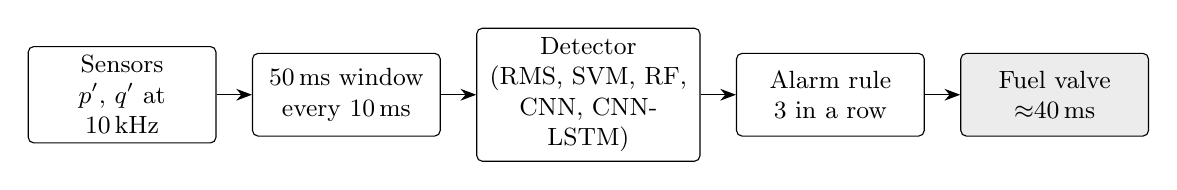
\begin{tikzpicture}[node distance=0.55cm and 0.45cm, box/.style={draw, rounded corners=2pt, align=center, minimum height=1.05cm, text width=2.15cm, font=\small}, >={Stealth[length=2mm]}]
\node[box] (s) {Sensors\\ $\pp$, $\qq$ at 10\,kHz};
\node[box, right=of s] (w) {50\,ms window\\ every 10\,ms};
\node[box, right=of w, text width=2.6cm] (d) {Detector\\ (RMS, SVM, RF,\\ CNN, CNN-LSTM)};
\node[box, right=of d] (a) {Alarm rule\\ 3 in a row};
\node[box, right=of a, fill=gray!15] (v) {Fuel valve\\ $\approx$40\,ms};
\draw[->] (s) -- (w); \draw[->] (w) -- (d); \draw[->] (d) -- (a); \draw[->] (a) -- (v);
\end{tikzpicture}
\caption{Proposed early-warning pipeline.}\label{fig:pipeline}
\end{figure}

What is new compared with the work in Section~\ref{sec:sota}:
\begin{itemize}
  \item fusion of $\pp$ and $\qq$, so the model can see the Rayleigh phase directly;
  \item explicit memory across bursts, to bridge the calm gaps;
  \item evaluation by warning time against a stated actuator delay;
  \item a common false-alarm budget for all detectors.
\end{itemize}

\subsection{Justification}
\begin{enumerate}
  \item \textbf{Physics of the driving.} By Eq.~\eqref{eq:rayleigh} and Eq.~\eqref{eq:ntau}, the phase between $\pp$ and $\qq$ moves towards the driving range \emph{before} the amplitude grows, because the amplitude only grows once driving beats damping. A detector that sees both signals can read this change while the pressure is still quiet.
  \item \textbf{Intermittency is a reliable precursor.} Turbulent combustors are known to reach instability through bursts \cite{nair2014}, so the bursting regime is a physically meaningful early-warning state rather than an arbitrary threshold.
  \item \textbf{Memory solves the calm-gap problem.} In the intermittent regime a 50\,ms window often falls between bursts and looks stable. A recurrent model that remembers recent bursts can keep the correct label through these gaps \cite{hochreiter1997}.
  \item \textbf{Real-time feasibility.} The inputs are short, one-dimensional windows and the networks are small (about $8\times10^4$ parameters), so inference fits comfortably inside the 10\,ms decision interval.
\end{enumerate}

%================================================== 5 MODEL & DATA
\section{Computational Model and Dataset}\label{sec:model}

\subsection{Why a simulation}
We searched for public data before building a model. The closest datasets are large recordings from an annular combustor \cite{faurebeaulieu_data} and short pressure recordings of stable, transient and limit-cycle combustion \cite{mirjan_data}. Neither contains synchronised pressure and heat-release signals over controlled $\phi$ sweeps, and neither gives the regime at every instant. We therefore used a reduced-order model to generate the main dataset, and used the second dataset for an external check (Section~\ref{sec:real}).

\subsection{Reduced-order combustor model}
We model the complex amplitude $a(t)$ of the quarter-wave mode with a stochastically forced oscillator in slow-flow form, in the spirit of \cite{noiray2013}:
\begin{equation}
  \frac{\mathrm{d}a}{\mathrm{d}t} = \left(\nu + \frac{\eta(t)}{1+|a|^2/a_\mathrm{lock}^2} + \mathrm{i}\,\Delta\omega\right)a + c_3|a|^2a - c_5|a|^4a + \sigma\,\xi(t).
  \label{eq:model}
\end{equation}
\begin{itemize}
  \item The mean growth rate follows from the Rayleigh criterion with an $n$--$\tau$ flame:
  \begin{equation}
    \nu(\phi) = \beta\cos\theta(\phi) - \alpha,\qquad \theta(\phi) = \frac{\theta_0 + k_\theta(\phi-0.55)}{U/U_\mathrm{ref}},
    \label{eq:nu}
  \end{equation}
  where $\beta$ is the flame driving gain, $\alpha$ the acoustic damping, and $\theta$ falls from about $105^\circ$ at $\phi=0.90$ to $30^\circ$ at $\phi=0.55$ (Figure~\ref{fig:thetanu}).
  \item $\eta(t)$ is an Ornstein--Uhlenbeck process with standard deviation $s_\nu$ and correlation time $\tau_\nu$, representing turbulent fluctuations of the flame gain. It is reduced once the flame locks onto the acoustic wave ($|a|>a_\mathrm{lock}$).
  \item The cubic and quintic terms make the bifurcation subcritical and saturate the limit cycle at about 2.4\,kPa.
  \item $\sigma\xi(t)$ is additive combustion noise.
\end{itemize}
Equation~\eqref{eq:model} is integrated with the Euler--Maruyama method at 10\,kHz.

The sensor signals are built from the amplitude and the carrier phase $\Phi(t)=2\pi\int f\,\mathrm{d}t$:
\begin{align}
  \pp(t) &= 0.97\,\big[\mathrm{Re}\{a e^{\mathrm{i}\Phi}\} + h_2\,\mathrm{Re}\{(a e^{\mathrm{i}\Phi})^2\} + p'_\mathrm{turb} + p'_\mathrm{mode2}\big]_{t-\tau_\mathrm{wg}} + \epsilon_p,\label{eq:p}\\
  \qq(t) &= \mathrm{Re}\{a\,e^{\mathrm{i}(\Phi-\theta)}\} + q'_\mathrm{flame} + \epsilon_q.\label{eq:q}
\end{align}
Here $p'_\mathrm{turb}$ is low-pass turbulent rumble, $p'_\mathrm{mode2}$ a weak second mode near 640\,Hz, and $\tau_\mathrm{wg}=0.5$\,ms the delay of the cooling tube between the wall and the transducer. Table~\ref{tab:params} lists the parameter values.

\begin{table}[H]\centering\small
\caption{Parameters of the reference rig. Each run perturbs flow, damping, noise and mode frequency (Table~\ref{tab:runs}).}\label{tab:params}
\begin{tabular}{llr}\toprule
Symbol & Meaning & Value\\\midrule
$\alpha$ & acoustic damping & 60.4\,s$^{-1}$ ($\pm$5\%)\\
$\beta$ & flame driving gain & 92.6\,s$^{-1}$\\
$\theta_0$, $k_\theta$ & phase lag at $\phi=0.55$, slope & $30^\circ$, $214.3^\circ$ per unit $\phi$\\
$c_3$, $c_5$ & nonlinear coefficients & 5.33\,s$^{-1}$kPa$^{-2}$, 0.889\,s$^{-1}$kPa$^{-4}$\\
$s_\nu$, $\tau_\nu$ & flame-gain fluctuation: std, correlation time & 25\,s$^{-1}$, 0.1\,s\\
$a_\mathrm{lock}$ & lock-in amplitude & 1.0\,kPa\\
$\sigma$ & additive forcing & 2.2 ($\pm$15\%)\\
$f_\mathrm{ref}$ & quarter-wave mode frequency & 205--215\,Hz\\
$\tau_\mathrm{wg}$ & waveguide delay & 0.5\,ms\\
$h_2$ & second-harmonic strength & 0.06\\
-- & turbulent rumble, sensor noise & 0.07\,kPa, 0.015\,kPa\\
\bottomrule\end{tabular}
\end{table}

\begin{figure}[H]\centering
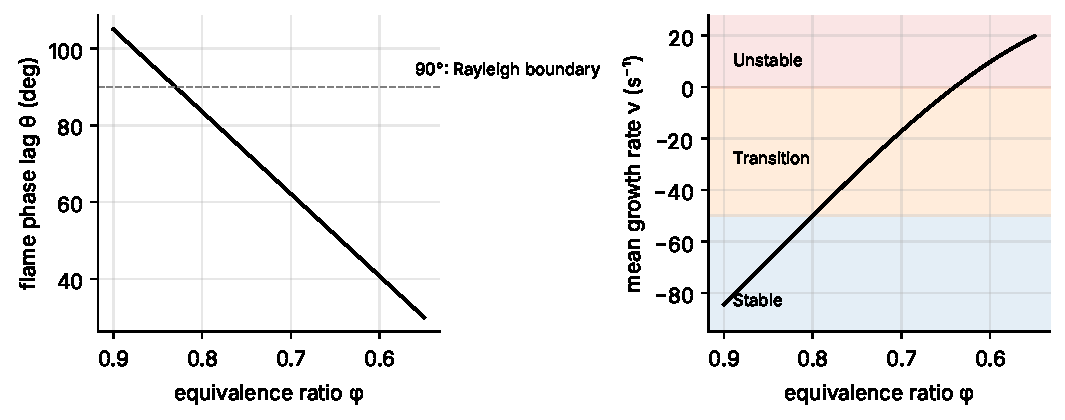
\includegraphics[width=0.95\textwidth]{theta_nu.pdf}
\caption{Model physics against equivalence ratio: flame phase lag $\theta$ (left) and mean growth rate $\nu$ with the three regime bands (right).}\label{fig:thetanu}
\end{figure}

\subsection{Ground-truth labelling}
The regime of each instant is set from the mean growth rate, not from the signal amplitude:
\begin{equation}
  \text{regime} = \begin{cases} \text{Stable} & \nu < -2s_\nu \\ \text{Transition} & -2s_\nu \le \nu < 0 \\ \text{Unstable} & \nu \ge 0 \end{cases}
  \label{eq:labels}
\end{equation}
Below $-2s_\nu$, turbulent fluctuations of the flame gain almost never overcome the damping. Between $-2s_\nu$ and 0 they intermittently push the net growth positive and create bursts. Above 0 the mean driving sustains the limit cycle. As a result, a calm window inside the transition is labelled Transition, which is what makes early warning a genuine prediction task.

\subsection{Experimental design}
Following the plan of our progress report, each \emph{slow sweep} lowers $\phi$ linearly from 0.90 to 0.55 in 30\,s. We simulated 15 sweeps with random variation in bulk flow ($\pm$6\%), damping ($\pm$5\%), noise ($\pm$15--25\%) and mode frequency (205--215\,Hz). Each signal is cut into 50\,ms windows with a 10\,ms stride, giving 2{,}996 windows per run and 44{,}940 in total. Runs are split as a whole into 11 training, 2 validation and 2 test sweeps (about 70/15/15), so that no window of a test run is ever seen in training. As a harder test of generalisation we also simulated 12 \emph{fast lean-outs}, in which $\phi$ falls from 0.86 to 0.58 in 1.5--4\,s. No model was trained on these. Table~\ref{tab:runs} lists the sweeps.

\begin{table}[H]\centering\footnotesize
\caption{The 15 slow sweeps: run-to-run variation, regime boundaries and number of windows per class.}\label{tab:runs}
\begin{tabular}{rlrrrrrrr}\toprule
Run & Split & Flow factor & $f_\mathrm{ref}$ (Hz) & $\phi_{S\to T}$ & $\phi_{T\to U}$ & Stable & Transition & Unstable \\\midrule
1 & train & 1.017 & 212.9 & 0.807 & 0.645 & 792 & 1392 & 812 \\
2 & train & 1.049 & 214.7 & 0.825 & 0.659 & 640 & 1422 & 934 \\
3 & train & 1.016 & 209.5 & 0.802 & 0.638 & 838 & 1405 & 753 \\
4 & train & 0.981 & 209.3 & 0.796 & 0.641 & 885 & 1335 & 776 \\
5 & train & 0.942 & 210.9 & 0.778 & 0.628 & 1042 & 1288 & 666 \\
6 & train & 0.992 & 213.0 & 0.800 & 0.643 & 850 & 1351 & 795 \\
7 & train & 0.981 & 214.0 & 0.785 & 0.625 & 982 & 1367 & 647 \\
8 & train & 0.978 & 212.0 & 0.788 & 0.631 & 955 & 1350 & 691 \\
9 & train & 0.999 & 210.5 & 0.798 & 0.638 & 868 & 1374 & 754 \\
10 & train & 0.985 & 211.8 & 0.795 & 0.638 & 893 & 1346 & 757 \\
11 & train & 1.009 & 210.2 & 0.805 & 0.644 & 810 & 1379 & 807 \\
12 & val & 1.000 & 205.6 & 0.807 & 0.649 & 793 & 1352 & 851 \\
13 & val & 0.983 & 209.2 & 0.789 & 0.631 & 944 & 1359 & 693 \\
14 & test & 1.055 & 214.5 & 0.814 & 0.643 & 731 & 1467 & 798 \\
15 & test & 0.943 & 209.9 & 0.781 & 0.631 & 1016 & 1283 & 697 \\
\midrule
\multicolumn{6}{l}{Total (44{,}940 windows)} & 13{,}039 & 20{,}470 & 11{,}431 \\
\bottomrule\end{tabular}
\end{table}

\subsection{Verification of the model}
Figures~\ref{fig:signals}--\ref{fig:rayleigh} show that the model reproduces the expected behaviour. In the stable regime $\pp$ is broadband noise. In the transition, bursts of the 210\,Hz mode grow and decay with calm gaps between them. In the unstable regime a steady limit cycle of about 2\,kPa RMS forms, and its spectrum is dominated by a single peak (Figure~\ref{fig:spectra}). Across all sweeps (Figure~\ref{fig:route}) bursts appear inside the transition band and the oscillation locks in near $\phi\approx0.64$. The measured Rayleigh index (Figure~\ref{fig:rayleigh}) is close to zero when stable ($-0.03$), positive in the transition ($+0.24$) and strongly positive in the limit cycle ($+0.74$), consistent with Eq.~\eqref{eq:rayleigh}.

\begin{figure}[H]\centering
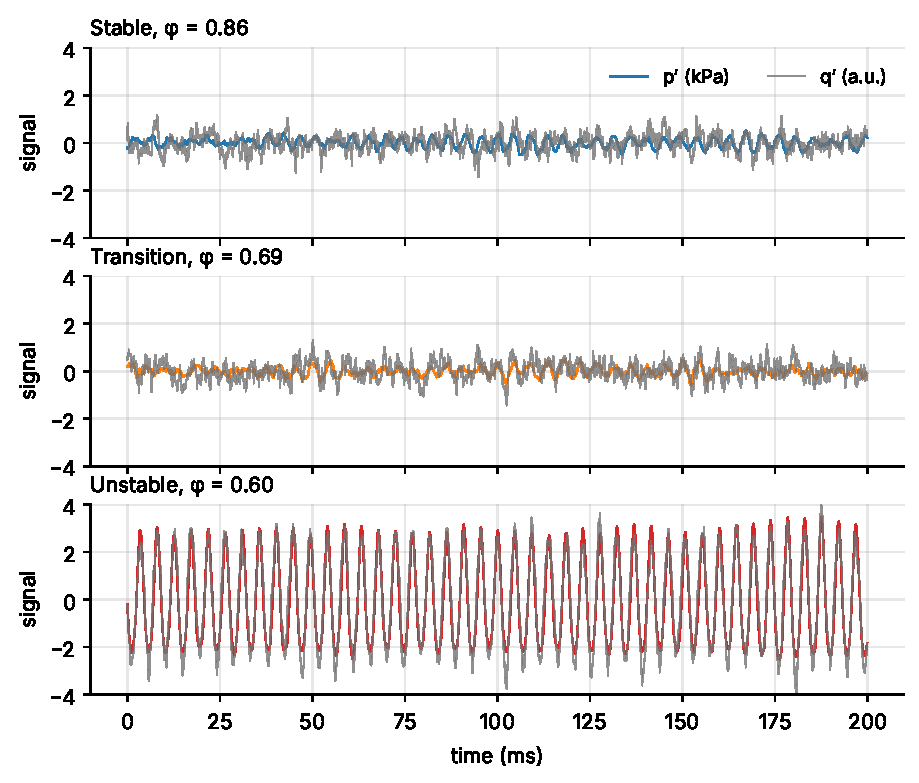
\includegraphics[width=0.9\textwidth]{signals.pdf}
\caption{Simulated pressure $\pp$ and flame light $\qq$ from a held-out sweep in the three regimes (200\,ms each).}\label{fig:signals}
\end{figure}

\begin{figure}[H]\centering
\begin{subfigure}{0.53\textwidth}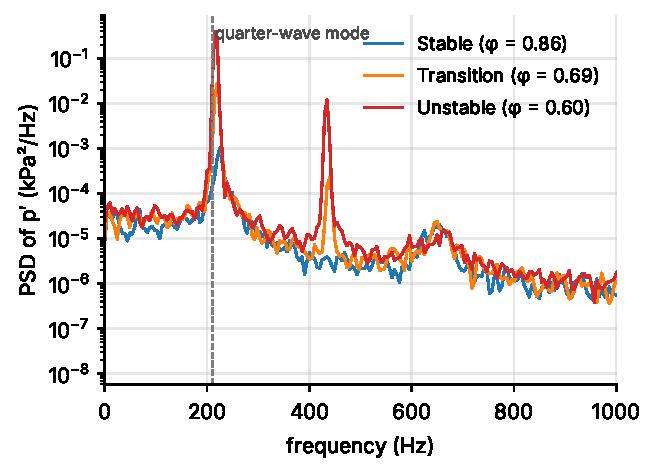
\includegraphics[width=\textwidth]{spectra.pdf}\caption{Power spectral density of $\pp$.}\label{fig:spectra}\end{subfigure}\hfill
\begin{subfigure}{0.44\textwidth}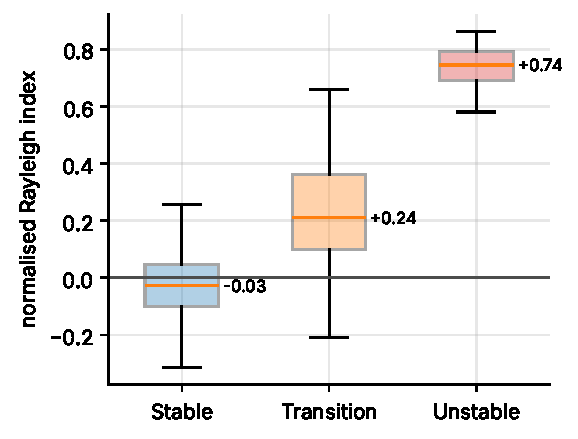
\includegraphics[width=\textwidth]{rayleigh.pdf}\caption{Normalised Rayleigh index per 50\,ms window.}\label{fig:rayleigh}\end{subfigure}
\caption{Spectral and energetic signatures of the three regimes (held-out and validation sweeps).}
\end{figure}

\begin{figure}[H]\centering
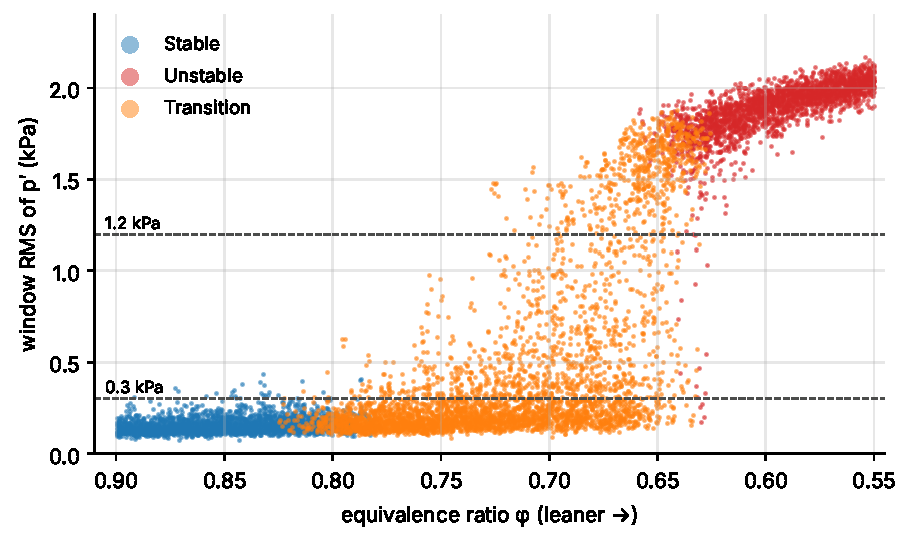
\includegraphics[width=0.8\textwidth]{route.pdf}
\caption{Route to instability: window RMS of $\pp$ against $\phi$ for all 15 sweeps, coloured by the true regime. Dashed lines are the 0.3 and 1.2\,kPa levels of the RMS rule.}\label{fig:route}
\end{figure}

\subsection{Assumptions and limitations of the model}
\begin{itemize}
  \item A single acoustic mode with a delayed flame response. Chemistry, three-dimensional flow and mode interaction are not modelled.
  \item The parameters were chosen so that the regime boundaries, frequency and amplitudes match our design targets (210\,Hz, 0.3/1.2\,kPa, $\phi$ 0.90$\to$0.55). They were not fitted to a specific experiment.
  \item The labels depend on the threshold $-2s_\nu$ in Eq.~\eqref{eq:labels}. Near this boundary bursts are rare, so a perfect detector cannot reach 100\% window accuracy.
\end{itemize}

%================================================== 6 METHODS
\section{Detection Methods}\label{sec:methods}

\subsection{Hand-crafted features}
For a window of $N=500$ samples with mean-removed pressure $p_i$, we compute five features.
\begin{align}
  p'_\mathrm{rms} &= \sqrt{\tfrac1N\textstyle\sum_i p_i^2}, &
  \kappa &= \frac{\tfrac1N\sum_i p_i^4}{p'^4_\mathrm{rms}},\\
  r_\mathrm{peak} &= \frac{\sum_{|f-f_\mathrm{pk}|\le30\,\mathrm{Hz}} |\hat P(f)|^2}{\sum_{20\le f\le2000\,\mathrm{Hz}} |\hat P(f)|^2}, &
  z &= \frac{\mathrm{ZCR}}{2f_\mathrm{pk}},\\
  \Delta\theta &= \Big|\arg\textstyle\sum_{|f-f_\mathrm{pk}|\le30} \hat P\hat Q^{*} - 2\pi f_\mathrm{pk}\tau_\mathrm{wg}\Big| .
\end{align}
Here $\hat P$, $\hat Q$ are 2048-point FFTs of Hann-windowed $\pp$ and $\qq$, $f_\mathrm{pk}$ is the dominant frequency between 80 and 2000\,Hz, and ZCR is the zero-crossing rate.
\begin{itemize}
  \item The kurtosis $\kappa$ is about 3 for Gaussian noise, about 1.5 for a pure sine, and higher for a burst growing out of quiet.
  \item $r_\mathrm{peak}$ measures how much of the energy sits in one tone.
  \item $z$ is close to 1 for a clean tone.
  \item $\Delta\theta$ is the Rayleigh phase angle, with the waveguide delay calibrated out.
\end{itemize}
Figure~\ref{fig:features} shows their distributions.

\begin{figure}[H]\centering
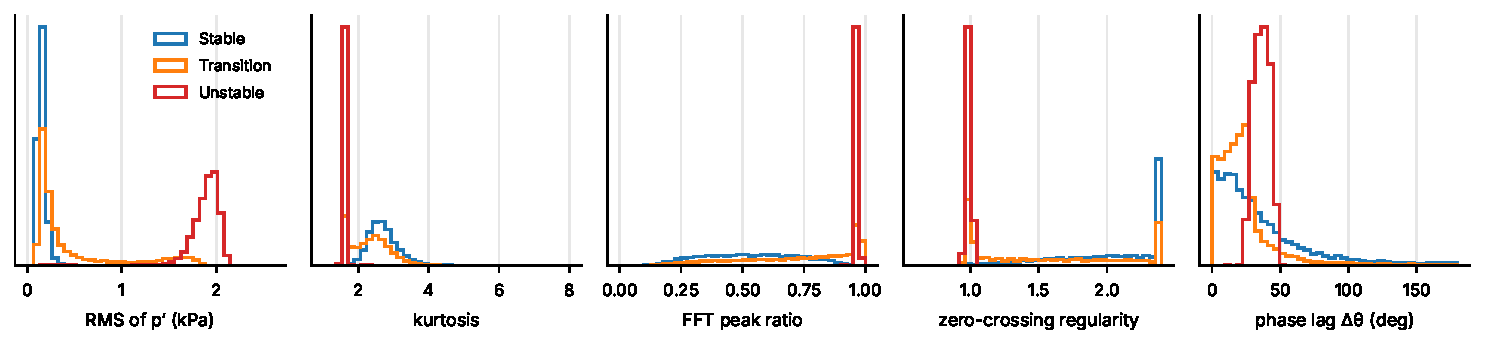
\includegraphics[width=\textwidth]{features.pdf}
\caption{Distributions of the five features per regime (training windows).}\label{fig:features}
\end{figure}

\subsection{Detectors}
\begin{enumerate}
  \item \textbf{RMS danger alarm}: unstable if $p'_\mathrm{rms}\ge1.2$\,kPa, otherwise stable (common practice).
  \item \textbf{RMS 3-level rule}: stable below 0.3\,kPa, transition from 0.3 to 1.2\,kPa, unstable above (rule of our progress report).
  \item \textbf{SVM}: RBF kernel, $C=10$, standardised features \cite{cortes1995}.
  \item \textbf{Random Forest}: 100 trees, minimum leaf size 3 \cite{breiman2001}.
  \item \textbf{RF + smoothing}: Random Forest probabilities averaged causally over the last 10 windows (100\,ms).
  \item \textbf{1D-CNN}: raw 500-sample $\pp$ window. Four strided 1-D convolutions (16, 32, 64, 64 filters; kernels 9, 7, 5, 5; stride 2), each followed by layer normalisation and GELU, then mean and max pooling, a 64-unit dense layer and a 3-class output.
  \item \textbf{CNN-LSTM ($\pp$)}: the same encoder applied to each of the last 16 windows (200\,ms of history), followed by an LSTM with 64 units \cite{hochreiter1997} and a dense output.
  \item \textbf{CNN-LSTM ($\pp+\qq$)}: as above, with two input channels per window (sensor fusion).
\end{enumerate}
The classical models use scikit-learn \cite{pedregosa2011}. The neural networks are written in JAX/Flax \cite{jax2018} and trained on a CPU for 3{,}000 steps with AdamW \cite{loshchilov2019} (peak learning rate $2\times10^{-3}$ with warm-up and cosine decay, weight decay $10^{-4}$, gradient clipping 1.0) and cross-entropy loss. The weights with the best validation accuracy are kept.

\subsection{Alarm logic and threshold tuning}
A probabilistic detector raises a non-stable decision only if $P(\text{T})+P(\text{U})>\tau$. It then chooses between Transition and Unstable by the larger probability. For each detector, $\tau$ is the smallest value that keeps the false-alarm rate on the two \emph{validation} sweeps at or below 5\% (values between 0.72 and 0.92). The alarm switches on after three consecutive non-stable decisions (30\,ms), which filters single turbulent puffs, and off after ten stable decisions.

%================================================== 7 METRICS
\section{Evaluation Metrics}\label{sec:metrics}
Let $y_k$ be the true regime of window $k$ and $\hat y_k$ the decision. With windows every $\Delta t=10$\,ms:
\begin{align}
  \text{Accuracy} &= \frac{\#\{k:\hat y_k=y_k\}}{\#\{k\}}, \qquad
  \text{Transition recall} = \frac{\#\{k: y_k=\mathrm T,\ \hat y_k\ne \mathrm S\}}{\#\{k: y_k=\mathrm T\}},\\
  \text{False-alarm rate} &= \frac{\#\{k: y_k=\mathrm S,\ \hat y_k\ne \mathrm S\}}{\#\{k: y_k=\mathrm S\}} .
\end{align}
Macro-F1 is the mean of the per-class F1 scores. \emph{Full instability} starts at the first window $k_\mathrm{on}$ where $p'_\mathrm{rms}\ge1.2$\,kPa and stays above it for at least 90\% of the following 300\,ms. If the alarm episode active at $k_\mathrm{on}$ started at $k_\mathrm{a}$, and the true transition began at $k_\mathrm{T}$, the warning time is
\begin{equation}
  L = \big(k_\mathrm{on} - \max(k_\mathrm a, k_\mathrm T)\big)\,\Delta t .
\end{equation}
If no alarm is active at onset, $L$ is minus the delay to the next alarm. Taking $\max(k_\mathrm a,k_\mathrm T)$ ensures that an alarm raised while the flame is still stable earns no warning credit; it counts as false alarms instead. We report the median and minimum of $L$ over runs and the number of runs with $L\ge40$\,ms, the actuator time. Computation time is measured for one decision on one CPU core, including feature extraction.

%================================================== 8 RESULTS
\section{Results}\label{sec:results}
All results in this section are \emph{demonstrated in simulation} on runs that were not used for training or threshold tuning.

\subsection{Overall comparison}
Table~\ref{tab:fast} gives the main comparison on the 12 fast lean-outs and Table~\ref{tab:slow} on the two held-out slow sweeps. The fusion CNN-LSTM is the most accurate detector in both scenarios (89.8\% and 87.5\%). On the fast runs its median warning is 1.15\,s, its worst run 620\,ms, and every run is warned at least 40\,ms ahead. The RMS danger alarm fires 20\,ms \emph{after} the onset of full instability in every run. Per-class recall and computation time are in Table~\ref{tab:latency}.

{\setlength{\tabcolsep}{4pt}\begin{table}[H]\centering\small
\caption{Results on the 12 unseen fast lean-out runs. Thresholds of the probabilistic detectors were tuned on the validation runs for at most 5\% false alarms.}\label{tab:fast}
\resizebox{\textwidth}{!}{\begin{tabular}{lrrrrrrr}\toprule
Detector & Acc. (\%) & Macro-F1 & Trans. caught (\%) & False alarms (\%) & Median warning & Worst run & Runs $\geq$40\,ms \\\midrule
RMS danger alarm (1.2\,kPa) & 69.4 & 0.549 & 0.0 & 0.0 & $-$20\,ms & $-$20\,ms & 0/12 \\
RMS 3-level rule & 76.2 & 0.692 & 23.4 & 0.5 & 210\,ms & 60\,ms & 12/12 \\
SVM (5 features) & 78.1 & 0.735 & 34.4 & 1.7 & 255\,ms & 50\,ms & 12/12 \\
Random Forest (5 features) & 78.5 & 0.741 & 35.6 & 2.2 & 275\,ms & 60\,ms & 12/12 \\
RF + 100\,ms smoothing & 79.2 & 0.753 & 38.8 & 0.8 & 245\,ms & 30\,ms & 11/12 \\
1D-CNN (raw $p'$) & 76.5 & 0.723 & 34.7 & 0.9 & 295\,ms & 50\,ms & 12/12 \\
CNN-LSTM ($p'$) & 68.8 & 0.670 & 42.1 & 0.0 & 365\,ms & 90\,ms & 12/12 \\
\textbf{CNN-LSTM ($p'+q'$)} & \textbf{89.8} & \textbf{0.892} & \textbf{82.8} & \textbf{6.9} & \textbf{1.15\,s} & \textbf{620\,ms} & \textbf{12/12} \\
\bottomrule\end{tabular}}
\end{table}}
{\setlength{\tabcolsep}{4pt}\begin{table}[H]\centering\small
\caption{Results on the two held-out slow sweeps (30\,s each), same operating point as Table~\ref{tab:fast}.}\label{tab:slow}
\resizebox{\textwidth}{!}{\begin{tabular}{lrrrrrrr}\toprule
Detector & Acc. (\%) & Macro-F1 & Trans. caught (\%) & False alarms (\%) & Median warning & Worst run & Runs $\geq$40\,ms \\\midrule
RMS danger alarm (1.2\,kPa) & 53.8 & 0.493 & 0.0 & 0.0 & $-$20\,ms & $-$20\,ms & 0/2 \\
RMS 3-level rule & 64.8 & 0.649 & 24.9 & 1.5 & 420\,ms & 150\,ms & 2/2 \\
SVM (5 features) & 69.5 & 0.719 & 39.0 & 1.8 & 905\,ms & 760\,ms & 2/2 \\
Random Forest (5 features) & 70.2 & 0.724 & 40.9 & 3.4 & 630\,ms & 500\,ms & 2/2 \\
RF + 100\,ms smoothing & 72.6 & 0.749 & 45.6 & 2.3 & 610\,ms & 500\,ms & 2/2 \\
1D-CNN (raw $p'$) & 63.6 & 0.651 & 32.9 & 1.0 & 430\,ms & 150\,ms & 2/2 \\
CNN-LSTM ($p'$) & 70.1 & 0.721 & 49.0 & 2.0 & 860\,ms & 680\,ms & 2/2 \\
\textbf{CNN-LSTM ($p'+q'$)} & \textbf{87.5} & \textbf{0.884} & \textbf{82.5} & \textbf{10.5} & \textbf{4.91\,s} & \textbf{4.64\,s} & \textbf{2/2} \\
\bottomrule\end{tabular}}
\end{table}}
\begin{table}[H]\centering\small
\caption{Per-class recall on the fast lean-outs and computation time per decision (one CPU core, feature extraction included).}\label{tab:latency}
\begin{tabular}{lrrrr}\toprule
Detector & Stable (\%) & Transition (\%) & Unstable (\%) & Time/decision (ms) \\\midrule
RMS danger alarm (1.2\,kPa) & 100.0 & 0.0 & 97.5 & $<$0.1 \\
RMS 3-level rule & 99.5 & 23.4 & 97.5 & $<$0.1 \\
SVM (5 features) & 98.3 & 34.4 & 95.1 & 0.67 \\
Random Forest (5 features) & 97.8 & 35.6 & 95.6 & 4.66 \\
RF + 100\,ms smoothing & 99.2 & 38.8 & 93.9 & 4.66 \\
1D-CNN (raw $p'$) & 99.1 & 34.7 & 90.4 & 0.44 \\
CNN-LSTM ($p'$) & 100.0 & 42.1 & 64.8 & 1.77 \\
CNN-LSTM ($p'+q'$) & 93.1 & 82.8 & 92.5 & 1.66 \\
\bottomrule\end{tabular}
\end{table}

\subsection{Warning time}
Figure~\ref{fig:lead} shows the warning time of every detector on each fast run. All other detectors give between 30 and 730\,ms on individual runs. The fusion model's warnings lie between 620 and 1{,}780\,ms. On these runs this is a median of 83\% (minimum 52\%) of the time actually spent in the transition. Figure~\ref{fig:replay} shows one run in detail: the RMS rule flickers on individual bursts, while the fusion model holds its alarm through the calm gaps.

\begin{figure}[H]\centering
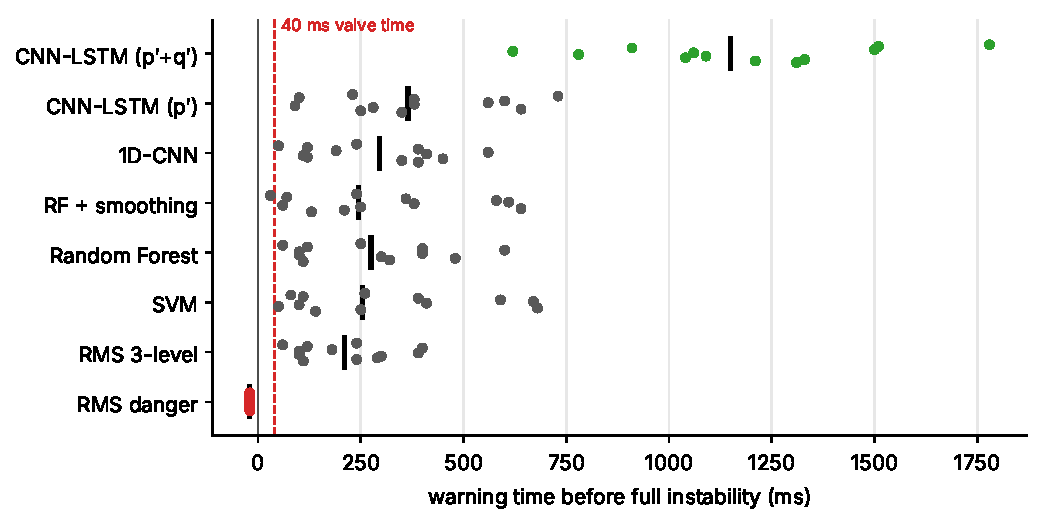
\includegraphics[width=0.85\textwidth]{leadtime.pdf}
\caption{Warning time per fast lean-out run (dots) and median (bar). Red dashed line: 40\,ms actuator time.}\label{fig:lead}
\end{figure}

\begin{figure}[H]\centering
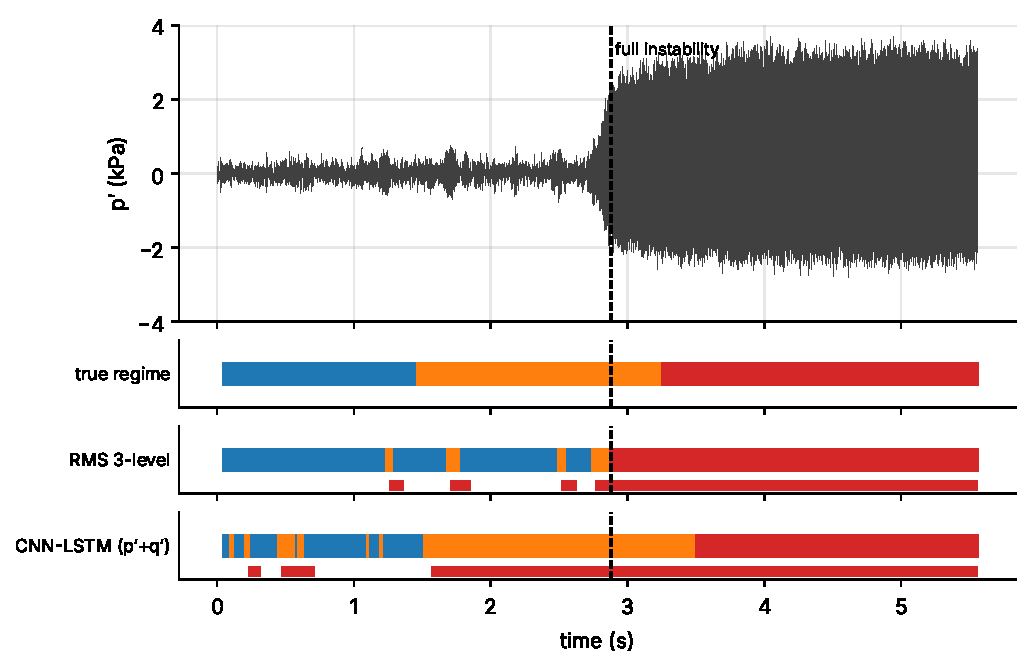
\includegraphics[width=0.88\textwidth]{replay101.pdf}
\caption{Fast lean-out run 101: pressure signal, true regime and decisions of the RMS rule and the fusion CNN-LSTM (blue stable, orange transition, red unstable). Red bars mark the alarm; the dashed line is the onset of full instability.}\label{fig:replay}
\end{figure}

\subsection{The quiet-gap problem}
Inside the true transition, 62\% of the windows fall in a calm gap (RMS below 0.3\,kPa). Table~\ref{tab:gap} and Figure~\ref{fig:gap} show that every detector catches almost all burst windows. Only the fusion model catches most gap windows (73\%, against 11\% for the Random Forest). Its decision also switches between stable and non-stable far less often than the Random Forest's (3.1 against 9.3 times per second of transition).

\begin{table}[H]\centering\small
\caption{Recall inside the true transition, split into windows containing a burst (RMS $\geq$ 0.3\,kPa) and windows in a calm gap (RMS $<$ 0.3\,kPa), slow sweeps. \textit{Flips} counts how often the decision switches between stable and non-stable per second of transition.}\label{tab:gap}
\begin{tabular}{lrrr}\toprule
Detector & Burst windows (\%) & Calm-gap windows (\%) & Flips per second \\\midrule
RMS danger alarm (1.2\,kPa) & 34 & 0 & 0.6 \\
RMS 3-level rule & 100 & 0 & 3.6 \\
SVM (5 features) & 90 & 11 & 10.5 \\
Random Forest (5 features) & 98 & 11 & 9.3 \\
RF + 100\,ms smoothing & 91 & 21 & 3.1 \\
1D-CNN (raw $p'$) & 94 & 6 & 6.4 \\
CNN-LSTM ($p'$) & 94 & 25 & 3.6 \\
CNN-LSTM ($p'+q'$) & 100 & 73 & 3.1 \\
\bottomrule\end{tabular}
\end{table}
\begin{figure}[H]\centering
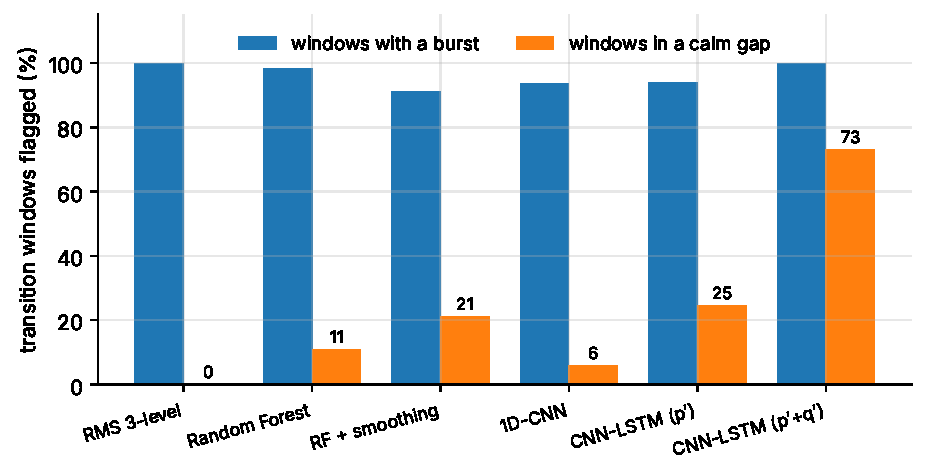
\includegraphics[width=0.8\textwidth]{quietgap.pdf}
\caption{Transition windows flagged, split into burst and calm-gap windows (slow sweeps). Numbers give the calm-gap recall.}\label{fig:gap}
\end{figure}

\subsection{Where the errors and false alarms are}
The confusion matrices (Figure~\ref{fig:cm}) show that the Random Forest labels 63\% of transition windows as stable, while the fusion model labels only 17\% as stable. In return it flags 7\% of stable windows (Random Forest: 2\%). Neither model confuses stable with unstable. Figure~\ref{fig:fard} shows where those false alarms occur. For the fusion model, 41\% of stable windows within 0.01 of $\phi$ above the true boundary are flagged, but only 3.4\% of those more than 0.04 away. Its false alarms are therefore mostly early calls just before the boundary.

\begin{figure}[H]\centering
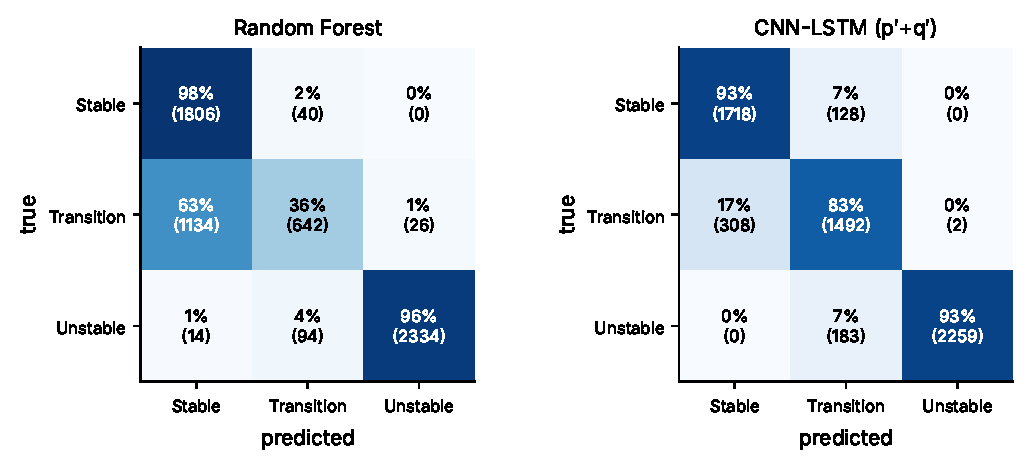
\includegraphics[width=0.82\textwidth]{confusion.pdf}
\caption{Confusion matrices on the fast lean-outs (row-normalised, counts in brackets).}\label{fig:cm}
\end{figure}

\begin{figure}[H]\centering
\begin{subfigure}{0.48\textwidth}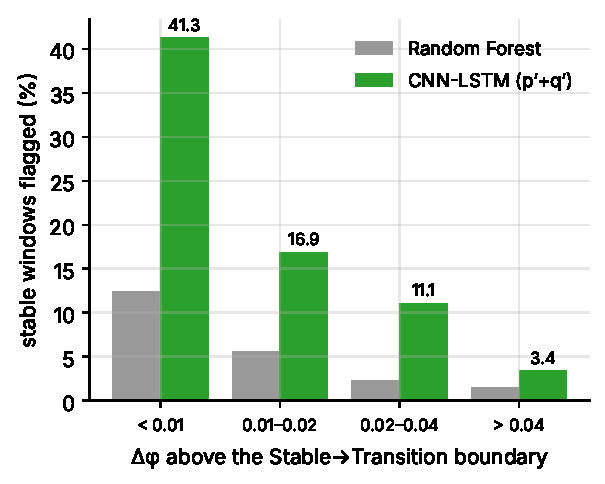
\includegraphics[width=\textwidth]{fardist.pdf}\caption{False alarms vs distance from the boundary (all 14 test runs).}\label{fig:fard}\end{subfigure}\hfill
\begin{subfigure}{0.49\textwidth}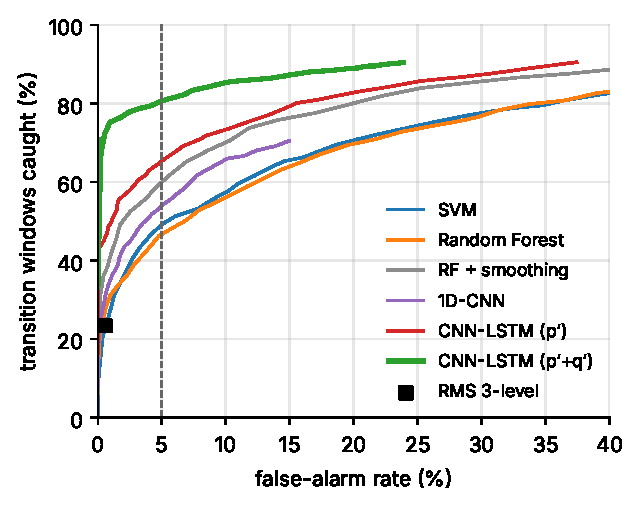
\includegraphics[width=\textwidth]{tradeoff.pdf}\caption{False-alarm rate vs transition recall as the threshold is swept (fast runs).}\label{fig:trade}\end{subfigure}
\caption{False-alarm behaviour of the detectors.}
\end{figure}

\subsection{Trade-off between false alarms and early detection}
Sweeping the decision threshold of each detector traces the curves of Figure~\ref{fig:trade}. At every false-alarm level the fusion model catches more transition windows than any other detector. At 5\% false alarms it catches 80\% of transition windows, while the other learned detectors catch 46--65\%. The RMS 3-level rule sits at a single point with very low recall.

\subsection{Features, window length and training}
The Random Forest relies most on the RMS (38\%), followed by kurtosis (19\%), FFT peak ratio (18\%), phase lag (16\%) and zero-crossing regularity (9\%) (Figure~\ref{fig:imp}). Longer windows smooth out noise and slightly improve accuracy (Table~\ref{tab:window}), but they react later to a new burst; 50\,ms (about ten cycles at 210\,Hz) is a reasonable compromise. Training curves and model sizes are in Figure~\ref{fig:train} and Table~\ref{tab:deep}.

\begin{figure}[H]\centering
\begin{subfigure}{0.47\textwidth}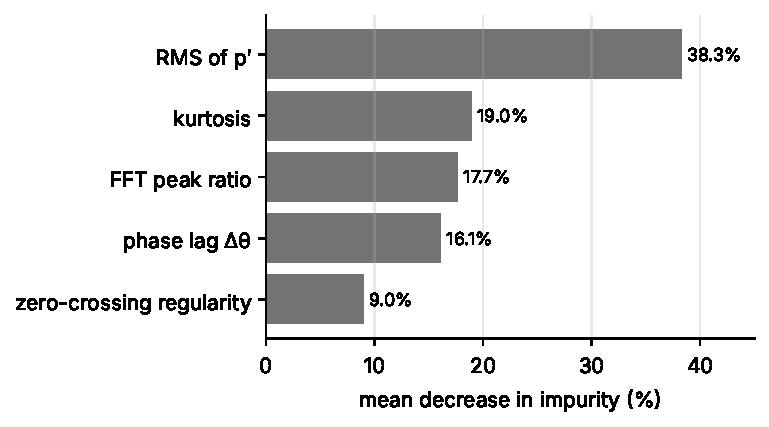
\includegraphics[width=\textwidth]{importance.pdf}\caption{Random Forest feature importance.}\label{fig:imp}\end{subfigure}\hfill
\begin{subfigure}{0.5\textwidth}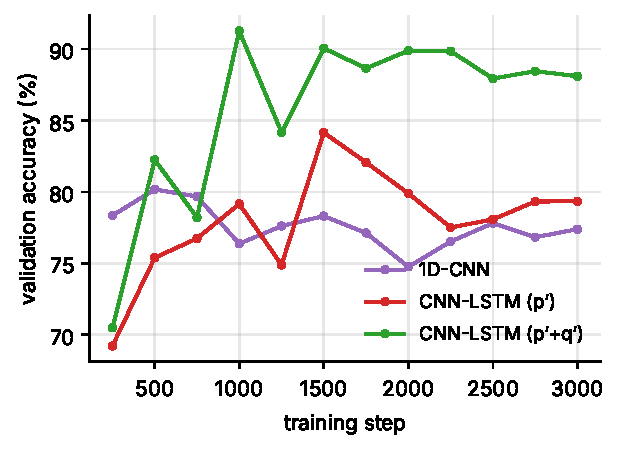
\includegraphics[width=\textwidth]{training.pdf}\caption{Validation accuracy during training.}\label{fig:train}\end{subfigure}
\caption{Feature importance and training behaviour.}
\end{figure}

\begin{table}[H]\centering\small
\caption{Effect of window length on the Random Forest (plain arg-max decisions).}\label{tab:window}
\begin{tabular}{rrrrr}\toprule
Window & Acc. slow (\%) & False alarms slow (\%) & Acc. fast (\%) & Median warning fast \\\midrule
30\,ms & 76.6 & 34.2 & 80.7 & 1.36\,s \\
50\,ms & 77.5 & 33.0 & 82.3 & 1.37\,s \\
100\,ms & 80.1 & 28.8 & 84.1 & 1.40\,s \\
\bottomrule\end{tabular}
\end{table}
\begin{table}[H]\centering\small
\caption{Deep models: size, training cost and best validation accuracy (plain arg-max).}\label{tab:deep}
\begin{tabular}{lrrrr}\toprule
Model & Parameters & Training time & Best val. acc. (\%) & Time per decision (ms) \\\midrule
1D-CNN (raw $p'$) & 47{,}587 & 4.6\,min & 80.2 & 0.44 \\
CNN-LSTM ($p'$) & 80{,}611 & 8.1\,min & 84.1 & 1.77 \\
CNN-LSTM ($p'+q'$) & 80{,}755 & 7.9\,min & 91.3 & 1.66 \\
\bottomrule\end{tabular}
\end{table}

%================================================== 9 DISCUSSION
\section{Discussion: Why the Detectors Behave as They Do}\label{sec:discussion}
\begin{description}[style=nextline]
  \item[RMS danger alarm.] A 1.2\,kPa level is reached only once the limit cycle has formed, so the alarm cannot anticipate it. It never recognises the transition and fires after onset in every run.
  \item[RMS 3-level rule.] It responds to any burst louder than 0.3\,kPa, which gives a few hundred milliseconds of warning. In every calm gap the RMS drops below 0.3\,kPa and the rule reverts to stable. It therefore catches none of the gap windows and only 23\% of all transition windows.
  \item[SVM and Random Forest.] Kurtosis and the spectral peak ratio let these models recognise the \emph{shape} of a burst, not just its loudness, so they recall more of the transition than the RMS rule. They still judge each window independently, which leaves 89\% of the gap windows undetected.
  \item[1D-CNN.] The network learns burst shapes directly from the raw signal and performs about as well as the feature models. Without memory it suffers from the same calm-gap problem.
  \item[CNN-LSTM ($\pp$ only).] Memory helps (25\% of gap windows), but from pressure alone the quiet windows of the early transition are almost indistinguishable from stable ones. To respect the 5\% false-alarm budget on validation, its threshold became strict ($\tau=0.915$). It therefore stays silent too often: zero false alarms, but the lowest accuracy (68.8\%).
  \item[CNN-LSTM ($\pp+\qq$).] With both channels the network can follow the phase relation between pressure and heat release. By Eq.~\eqref{eq:nu} this phase shifts smoothly towards driving as the mixture leans, even during quiet epochs, so it carries information that loudness does not. Combined with memory, the alarm comes early and stays on through the gaps. The validation accuracy rose from 84.1\% to 91.3\% with only 144 extra parameters (one extra input channel), so the gain comes from the information in $\qq$, not from model size.
\end{description}

The price of earlier warning is a higher false-alarm rate on the test runs (6.9\% on the fast runs, 10.5\% on the slow sweeps) than the 5\% chosen on validation. Two reasons explain this. The validation set contains only two runs, so the threshold has some sampling error. More importantly, the false alarms are concentrated just before the labelled boundary, where bursts are already physically possible. In a safety system such early calls are arguably acceptable, but the threshold should be re-tuned on more validation data.

%================================================== 10 REAL DATA
\section{Validation on Real Combustor Recordings}\label{sec:real}
We used 42 public pressure recordings (14 stable, 14 transient and 14 limit-cycle; 0.5\,s each at 10\,kHz) from an open-source student project \cite{mirjan_data}. Their origin is not fully documented and they contain no heat-release channel. We cut them into 1{,}932 windows of 50\,ms with the same feature code and dropped the phase feature. Their dominant frequencies (about 350--400\,Hz and 1.1\,kHz) differ from our 210\,Hz mode (Figure~\ref{fig:real}).

Two experiments were run (Table~\ref{tab:real}). First, a Random Forest trained on the recordings themselves with 7-fold cross-validation grouped by recording reached 94.1\% window accuracy and classified every recording correctly by majority vote. This shows that the features separate real regimes well. Second, a Random Forest trained only on our simulation reached 71.6\%, using rig-independent features in which the RMS is divided by the rig's stable baseline. It recognised stable and limit-cycle recordings but called many transient windows unstable, because the real bursts are louder relative to the baseline than in our model. This cross-rig drop is the main argument for calibrating the detector on data from the target engine.

\begin{figure}[H]\centering
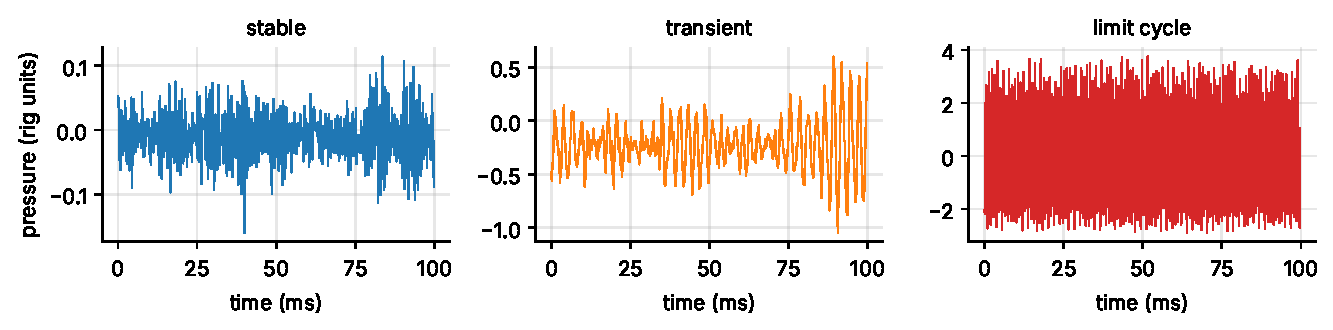
\includegraphics[width=0.95\textwidth]{realdata.pdf}
\caption{Example public recordings: stable, transient and limit cycle (100\,ms each).}\label{fig:real}
\end{figure}
\begin{table}[H]\centering\small
\caption{Window accuracy on the 42 public combustor recordings (1{,}932 windows of 50\,ms), overall and per true class.}\label{tab:real}
\begin{tabular}{lrrrr}\toprule
Model & Overall (\%) & Stable (\%) & Transient (\%) & Limit cyc. (\%) \\\midrule
RF trained on recordings (grouped CV) & 94.1 & 93.5 & 91.5 & 97.4 \\
RF trained on simulation (zero-shot) & 71.6 & 63.5 & 51.2 & 100.0 \\
RMS 3-level rule & 74.9 & 100.0 & 24.7 & 100.0 \\
\bottomrule\end{tabular}
\end{table}

%================================================== 11 EXPECTED + IMPACT
\section{Expected Results and Potential Impact}\label{sec:expected}
The following are \emph{expectations} supported by our analysis. They have not been demonstrated on a real engine.
\begin{itemize}
  \item \textbf{Accuracy after calibration.} With a few minutes of labelled data from the target rig, we expect accuracy close to the 94\% obtained on the real recordings, rather than the 72\% of the zero-shot transfer.
  \item \textbf{Warning time.} On the fast lean-outs the fusion model's warning covered a median of 83\% (at least 52\%) of the time spent in transition. For an engine whose intermittent phase lasts about a second, we therefore expect several hundred milliseconds of warning, comfortably more than a 40\,ms actuator.
  \item \textbf{Hardware.} At 1.7\,ms per decision on one CPU core, the detector should run in real time on an embedded processor with one pressure transducer and one photodiode. No high-speed camera is required.
  \item \textbf{Main risk.} Different chamber geometries, mode frequencies or sensor positions will require retraining, and a longer validation period is needed to set the threshold reliably.
\end{itemize}
If these expectations hold, the approach could (i) protect engines during development testing by triggering a shutdown or fuel redistribution before damage occurs, (ii) let combustors operate leaner, with lower NO$_x$ and higher efficiency, closer to the stability boundary with a safety net, and (iii) reduce the cost of instability monitoring.

%================================================== 12 LIMITATIONS
\section{Limitations and Future Work}
\begin{itemize}
  \item The main dataset is simulated with a single-mode model whose parameters match design targets rather than measurements. Validation on an instrumented rig with synchronised $\pp$ and $\qq$ is the most important next step.
  \item Only 42 short real recordings were available, without heat release or time history. Warning time could not be measured on real data.
  \item The optional flame-image (2D-CNN) track of our original plan was not pursued, as no camera data were available.
  \item The threshold was tuned on two validation runs. More validation data, or a calibrated probabilistic output, would make the false-alarm rate more predictable.
  \item Future work includes domain adaptation between rigs, testing with multiple modes, and closing the loop with a simulated actuator to measure how much warning is needed to actually suppress the instability.
\end{itemize}

%================================================== 13 CONTRIBUTIONS
\section{Individual Contributions}
\begin{table}[H]\centering\small
\caption{Individual contributions.}\label{tab:contrib}
\begin{tabular}{L{4.6cm}L{10cm}}\toprule
Member & Contribution\\\midrule
Pawan Sharma (23AE10024) & Reduced-order combustor model and dataset generation; 1D-CNN and CNN-LSTM models; interactive demonstration website\\
Harshvardhan Singh Chauhan (23AE30007) & Feature extraction; SVM and Random Forest baselines; window-length study; evaluation method (alarm rule, warning time, threshold tuning)\\
Vedaant Gupta (23AE3AI46) & Real-data validation; quiet-gap and false-alarm analysis; literature review; report and presentation\\
\bottomrule\end{tabular}
\end{table}

%================================================== 14 CONCLUSION
\section{Conclusion}
We framed early detection of thermoacoustic instability as a three-class problem on 50\,ms windows of pressure and flame-light data, and built a reduced-order combustor model that reproduces the intermittency route. Under a common false-alarm budget, a hybrid CNN-LSTM that fuses $\pp$ and $\qq$ gave a median warning of 1.15\,s on unseen fast lean-outs, against 0.21\,s for an RMS rule and no warning for a 1.2\,kPa danger alarm, with 1.7\,ms computation per decision. Two ingredients explain the improvement: the phase between pressure and heat release, which is the Rayleigh driving itself, and memory that bridges the calm gaps between bursts. A check on real recordings confirmed that the features separate real regimes but also showed that models must be calibrated for each engine. The approach is a promising, low-cost route to giving combustion controllers the time they need.

\bibliographystyle{unsrtnat}
\bibliography{refs}

%================================================== APPENDIX
\appendix
\section{Additional Results: Plain Arg-max Decisions}
Without threshold tuning, the probabilistic models flag many stable windows. This inflates both transition recall and warning time and shows why a common false-alarm budget is needed for a fair comparison.
{\setlength{\tabcolsep}{4pt}\begin{table}[H]\centering\small
\caption{Fast lean-outs with plain arg-max decisions (no threshold tuning). False alarms are much higher, which also inflates warning time.}\label{tab:defaultfast}
\resizebox{\textwidth}{!}{\begin{tabular}{lrrrrrrr}\toprule
Detector & Acc. (\%) & Macro-F1 & Trans. caught (\%) & False alarms (\%) & Median warning & Worst run & Runs $\geq$40\,ms \\\midrule
RMS danger alarm (1.2\,kPa) & 69.4 & 0.549 & 0.0 & 0.0 & $-$20\,ms & $-$20\,ms & 0/12 \\
RMS 3-level rule & 76.2 & 0.692 & 23.4 & 0.5 & 210\,ms & 60\,ms & 12/12 \\
SVM (5 features) & 82.0 & 0.805 & 78.2 & 31.7 & 1.37\,s & 320\,ms & 12/12 \\
Random Forest (5 features) & 82.3 & 0.809 & 77.9 & 30.8 & 1.37\,s & 340\,ms & 12/12 \\
RF + 100\,ms smoothing & 85.2 & 0.842 & 83.4 & 24.6 & 1.23\,s & 280\,ms & 12/12 \\
1D-CNN (raw $p'$) & 81.2 & 0.792 & 55.0 & 5.5 & 985\,ms & 120\,ms & 12/12 \\
CNN-LSTM ($p'$) & 75.0 & 0.754 & 76.9 & 13.3 & 1.15\,s & 290\,ms & 12/12 \\
\textbf{CNN-LSTM ($p'+q'$)} & \textbf{88.7} & \textbf{0.881} & \textbf{87.2} & \textbf{14.8} & \textbf{1.22\,s} & \textbf{620\,ms} & \textbf{12/12} \\
\bottomrule\end{tabular}}
\end{table}}
{\setlength{\tabcolsep}{4pt}\begin{table}[H]\centering\small
\caption{Slow sweeps with plain arg-max decisions.}\label{tab:defaultslow}
\resizebox{\textwidth}{!}{\begin{tabular}{lrrrrrrr}\toprule
Detector & Acc. (\%) & Macro-F1 & Trans. caught (\%) & False alarms (\%) & Median warning & Worst run & Runs $\geq$40\,ms \\\midrule
RMS danger alarm (1.2\,kPa) & 53.8 & 0.493 & 0.0 & 0.0 & $-$20\,ms & $-$20\,ms & 0/2 \\
RMS 3-level rule & 64.8 & 0.649 & 24.9 & 1.5 & 420\,ms & 150\,ms & 2/2 \\
SVM (5 features) & 78.2 & 0.793 & 77.8 & 33.3 & 5.25\,s & 4.51\,s & 2/2 \\
Random Forest (5 features) & 77.5 & 0.787 & 75.7 & 33.0 & 5.22\,s & 4.51\,s & 2/2 \\
RF + 100\,ms smoothing & 81.5 & 0.824 & 81.1 & 27.6 & 2.91\,s & 1.36\,s & 2/2 \\
1D-CNN (raw $p'$) & 68.9 & 0.706 & 46.4 & 4.1 & 920\,ms & 490\,ms & 2/2 \\
CNN-LSTM ($p'$) & 77.1 & 0.782 & 72.6 & 15.3 & 4.42\,s & 4.36\,s & 2/2 \\
\textbf{CNN-LSTM ($p'+q'$)} & \textbf{86.9} & \textbf{0.876} & \textbf{88.1} & \textbf{21.2} & \textbf{5.25\,s} & \textbf{4.65\,s} & \textbf{2/2} \\
\bottomrule\end{tabular}}
\end{table}}

\section{Core of the Simulator}
The slow-flow integration of Eq.~\eqref{eq:model}, as implemented in \texttt{simulator.py}:
\begin{lstlisting}[language=Python]
rho = np.exp(-DT / P.tau_nu)                       # flame-gain fluctuation (OU process)
eta = lfilter([np.sqrt(1 - rho*rho)], [1, -rho], rng.standard_normal(n)) * P.s_nu
inv_lock2 = 1.0 / P.a_lock**2
for k in range(n):
    r2 = z.real*z.real + z.imag*z.imag
    z = z + ((nu[k] + eta[k]/(1.0 + r2*inv_lock2) + 1j*dw)
             + c3*r2 - c5*r2*r2) * z * DT + noise[k]
    a[k] = z
\end{lstlisting}

\section{Reproducibility}
All code, data generation and figures can be reproduced with:
\begin{lstlisting}
python make_dataset.py        # 15 slow sweeps + 12 fast lean-outs
python train_classical.py     # RMS rules, SVM, Random Forest, window study
python train_deep.py cnn      # also: lstm_p, lstm_pq
python evaluate.py            # thresholds, metrics, quiet-gap analysis
python real_check.py          # public recordings
\end{lstlisting}
Total run time is about 25\,minutes on a two-core laptop CPU.

\end{document}
